% !TeX spellcheck = de_DE
\section{Lean Start-up und Pitching}
\subsection{Lean vs. Traditional}
\begin{multicols}{2}
	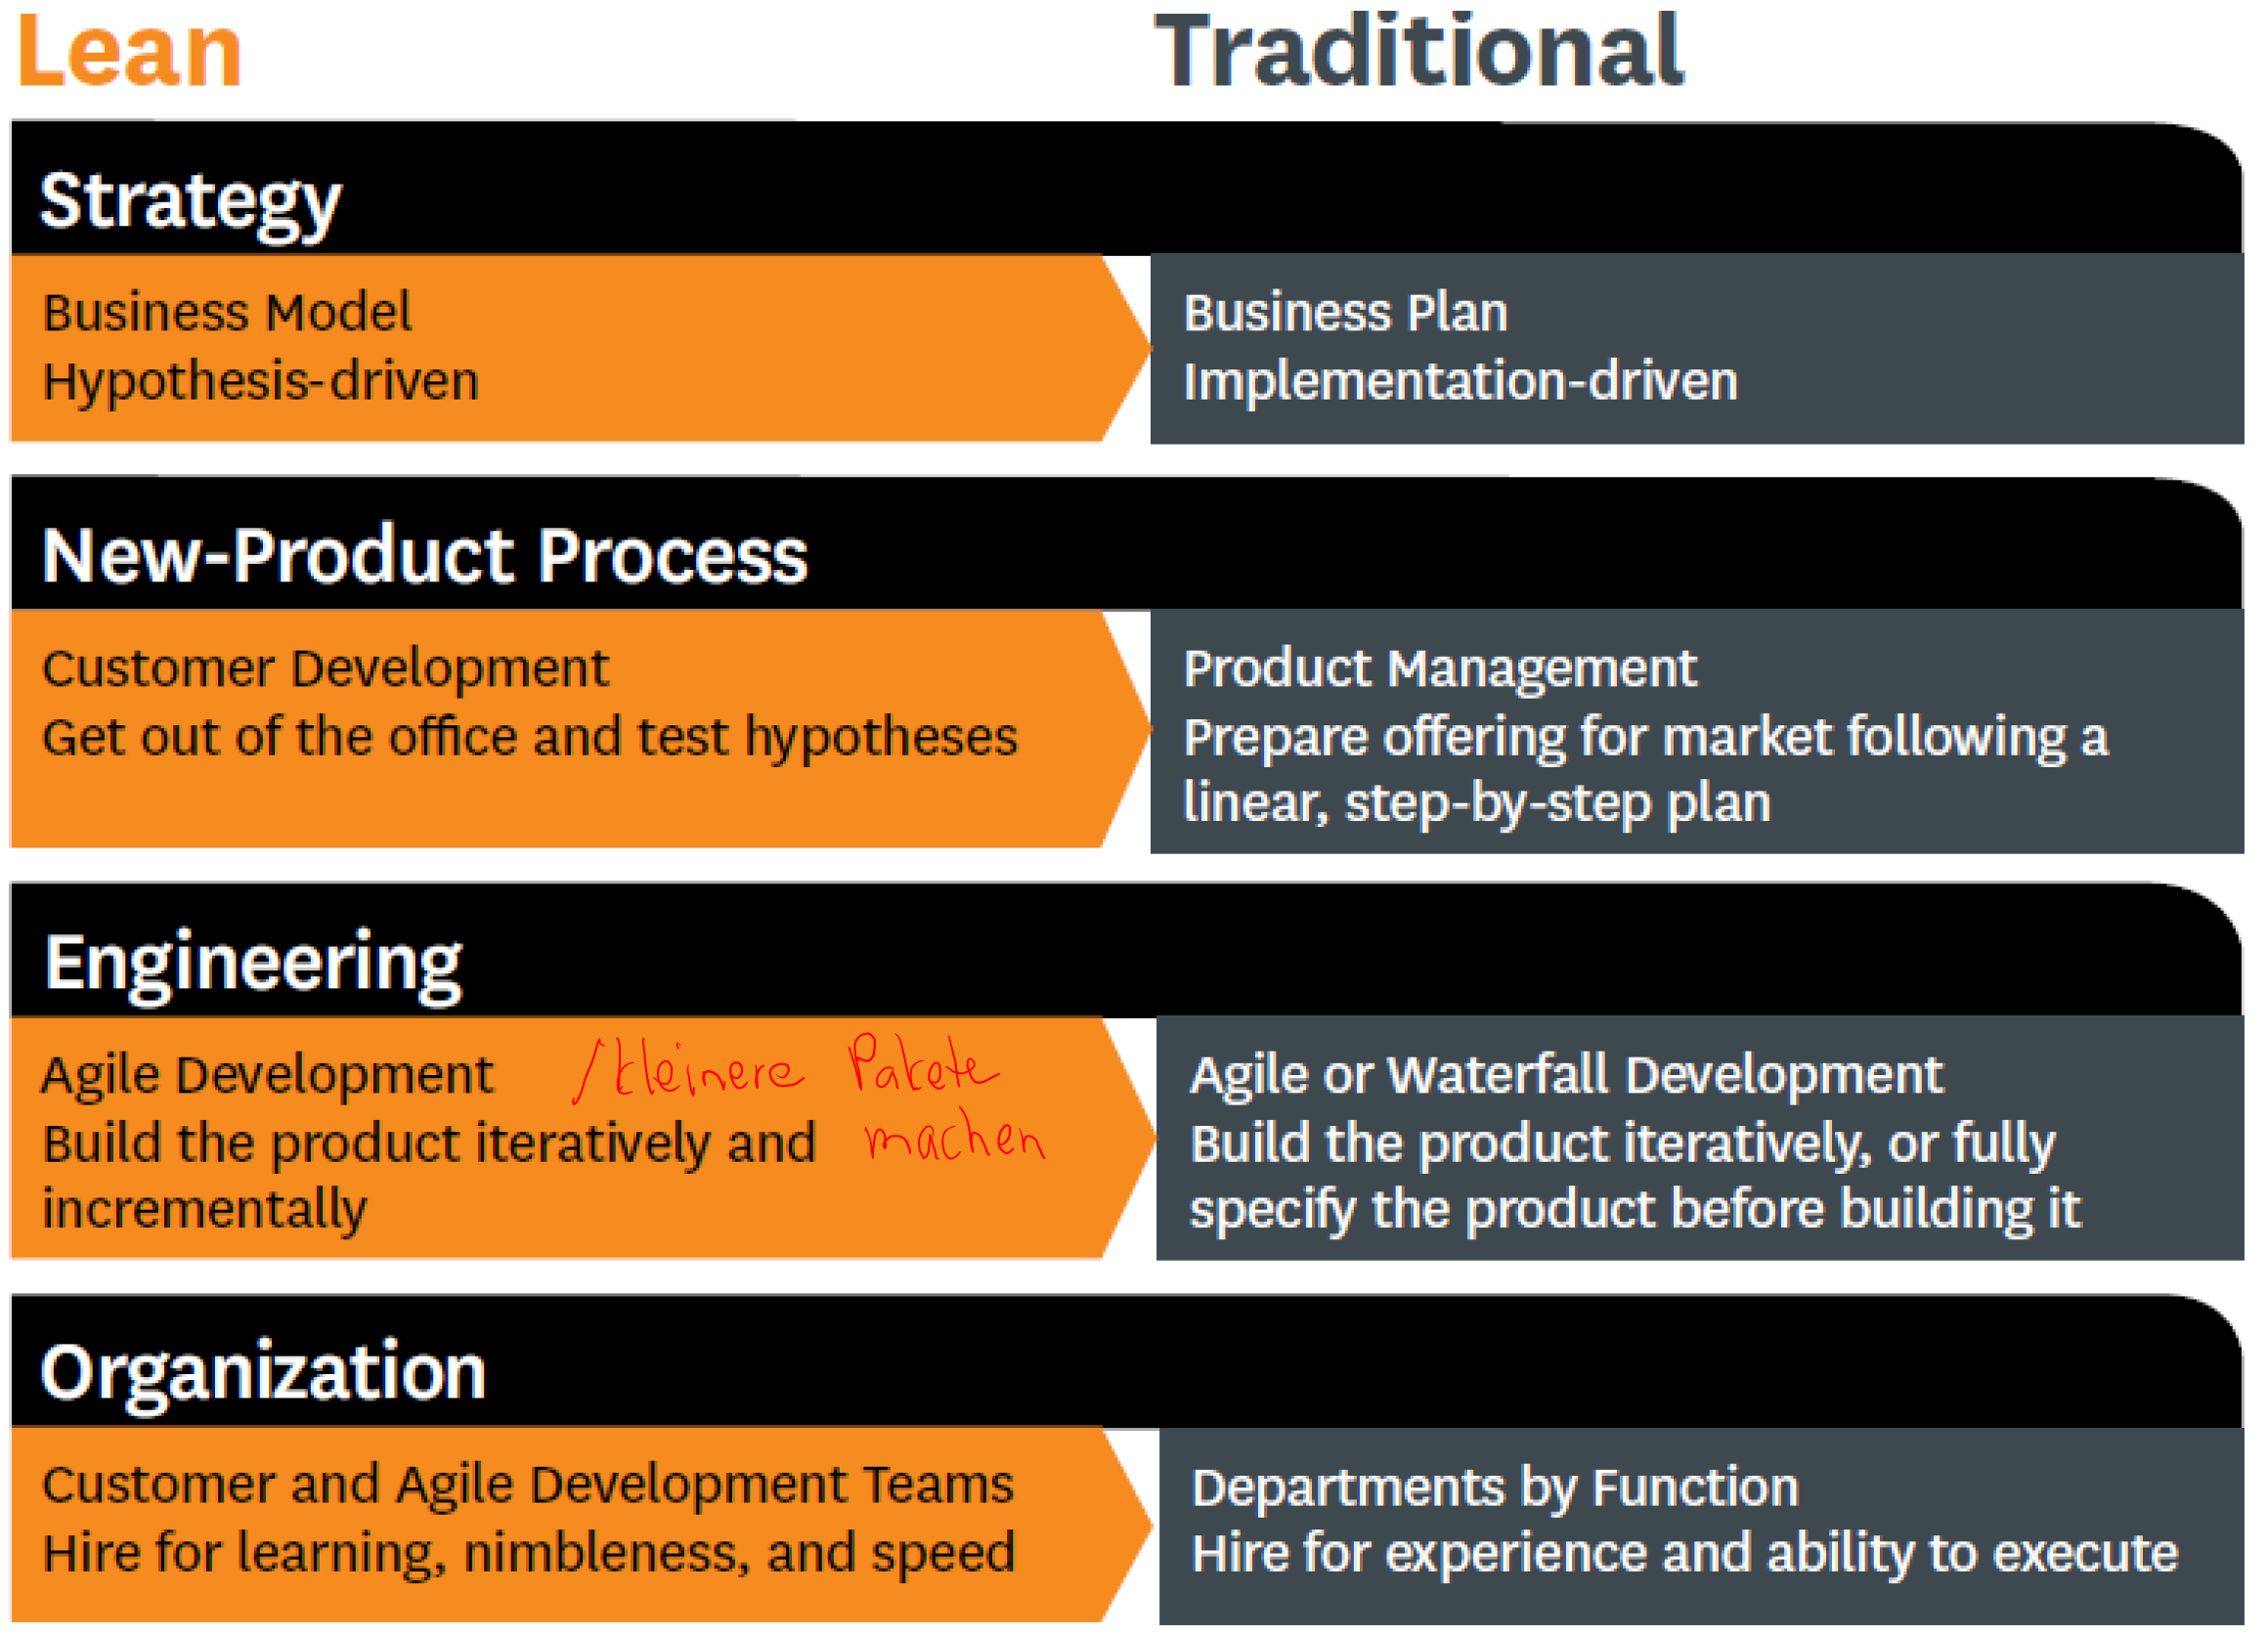
\includegraphics[width=1\linewidth]{images/lean}
	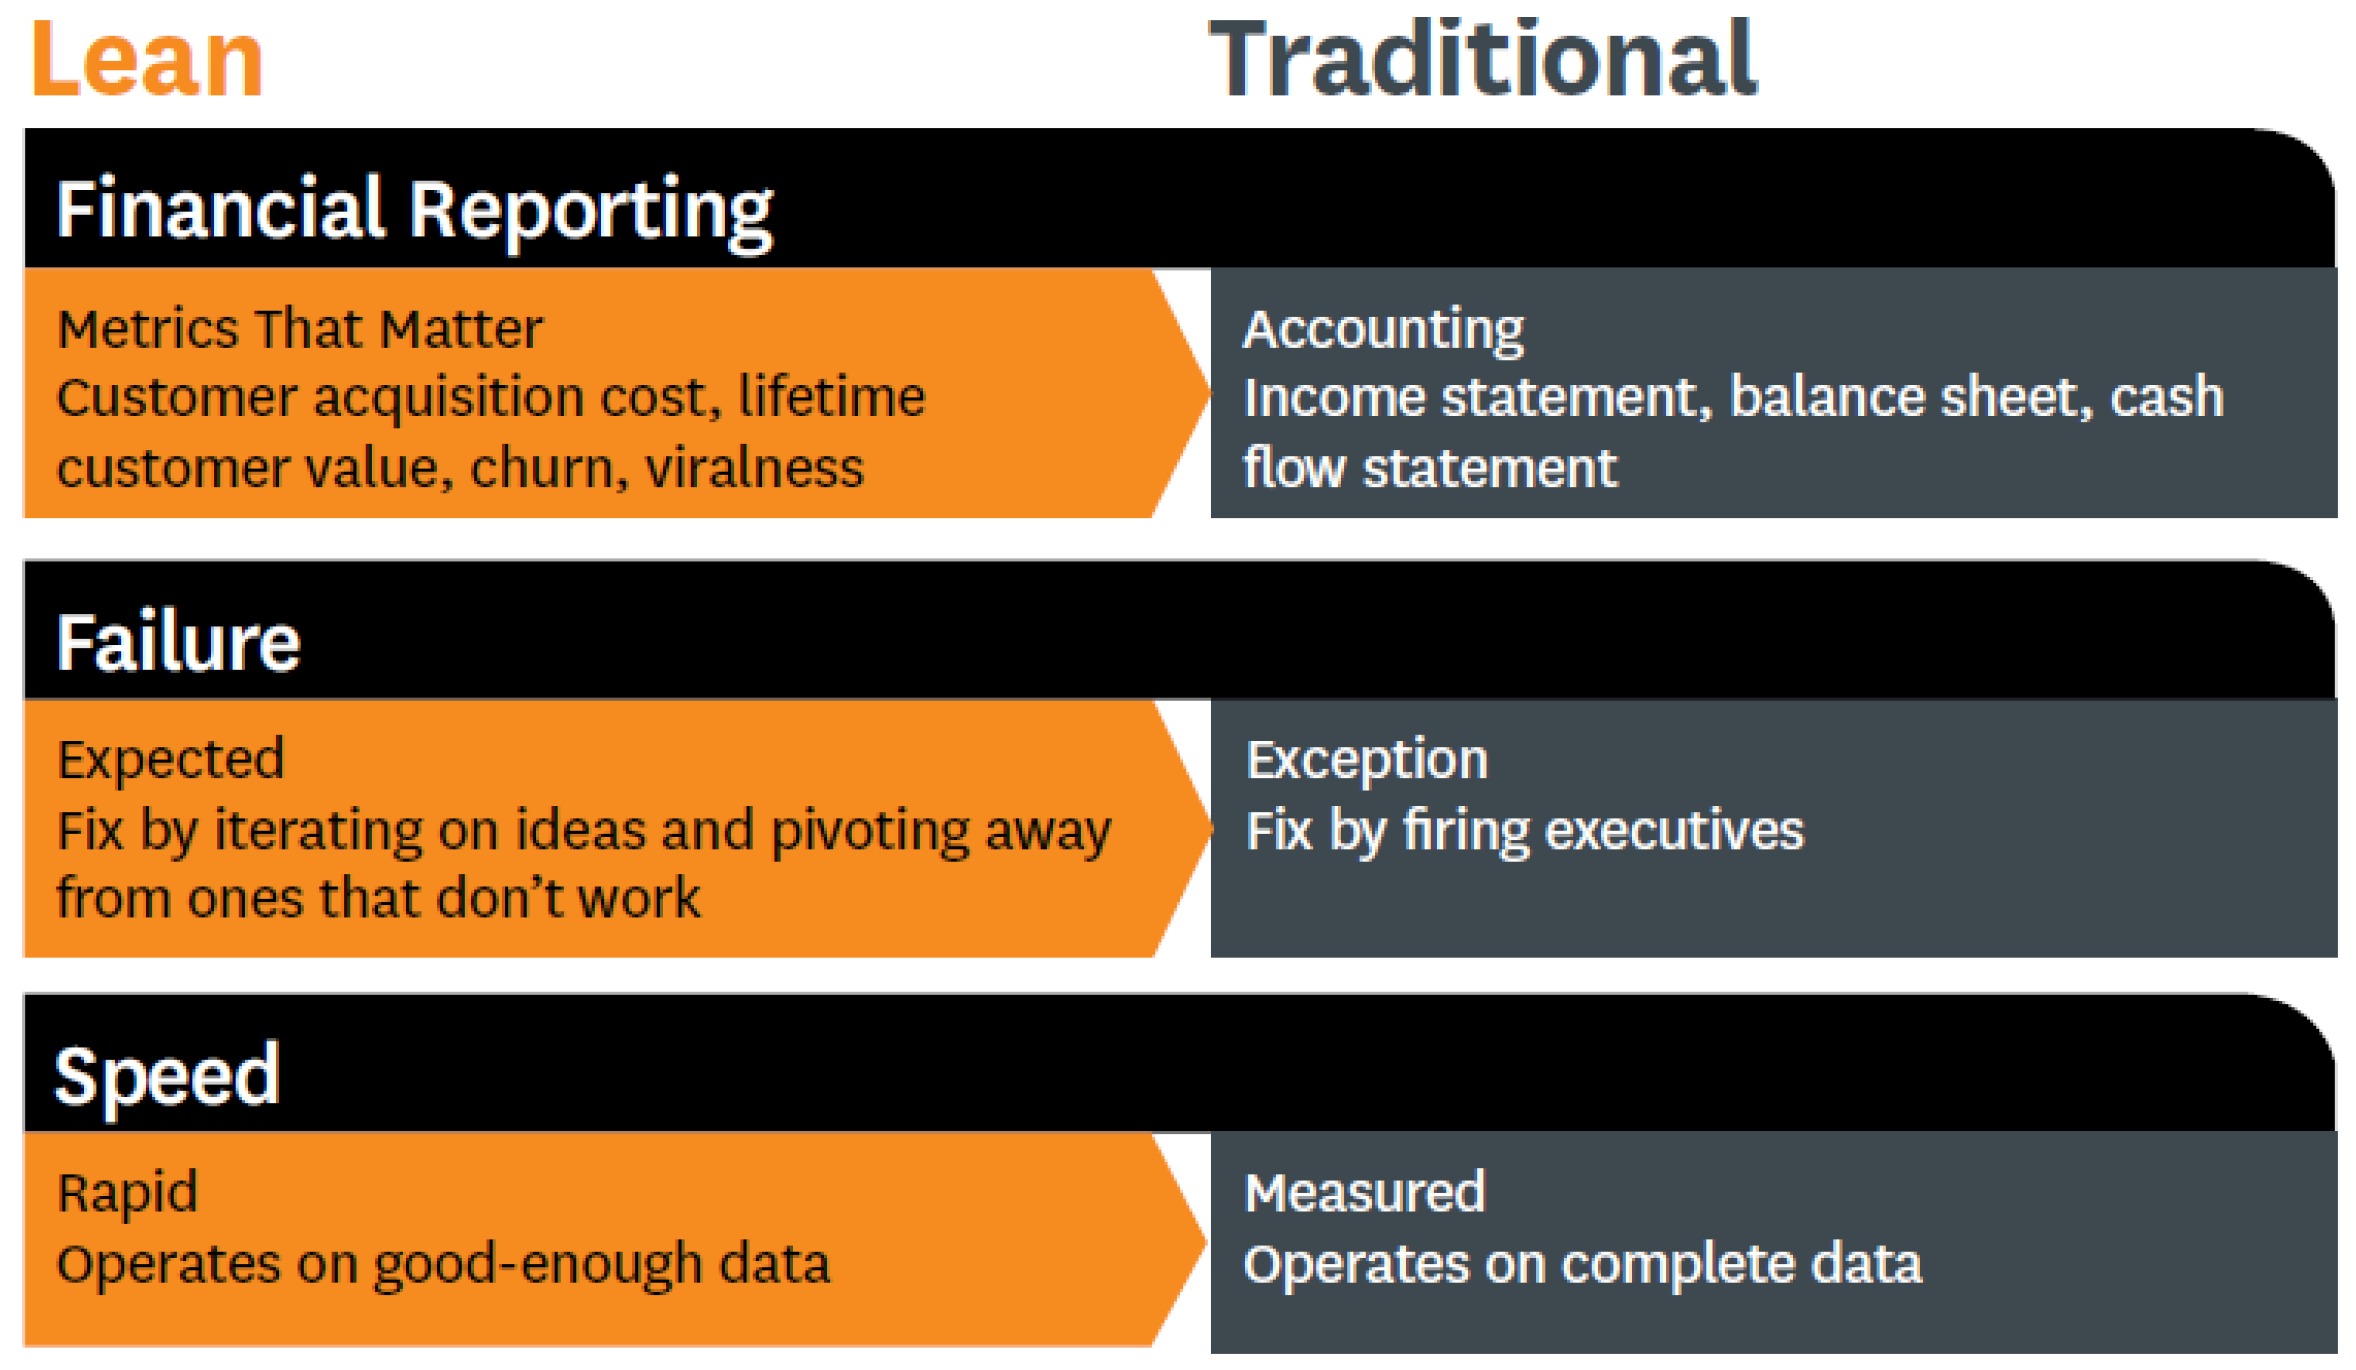
\includegraphics[width=1\linewidth]{images/lean_2}
\end{multicols}

\subsection{Lean}
Too many technology-driven startups spend weeks and months working on a product without ever speaking with a prospective client. By applying the lean startup methdology, you can:
\begin{itemize}
	\item Minimize risk
	\item Maximize success (learning)
	\item Receive quick feedback
	\item Reduce overhead
	\item Make measurable progress
\end{itemize}

\subsubsection{Vorgehen}
\begin{multicols}{2}
	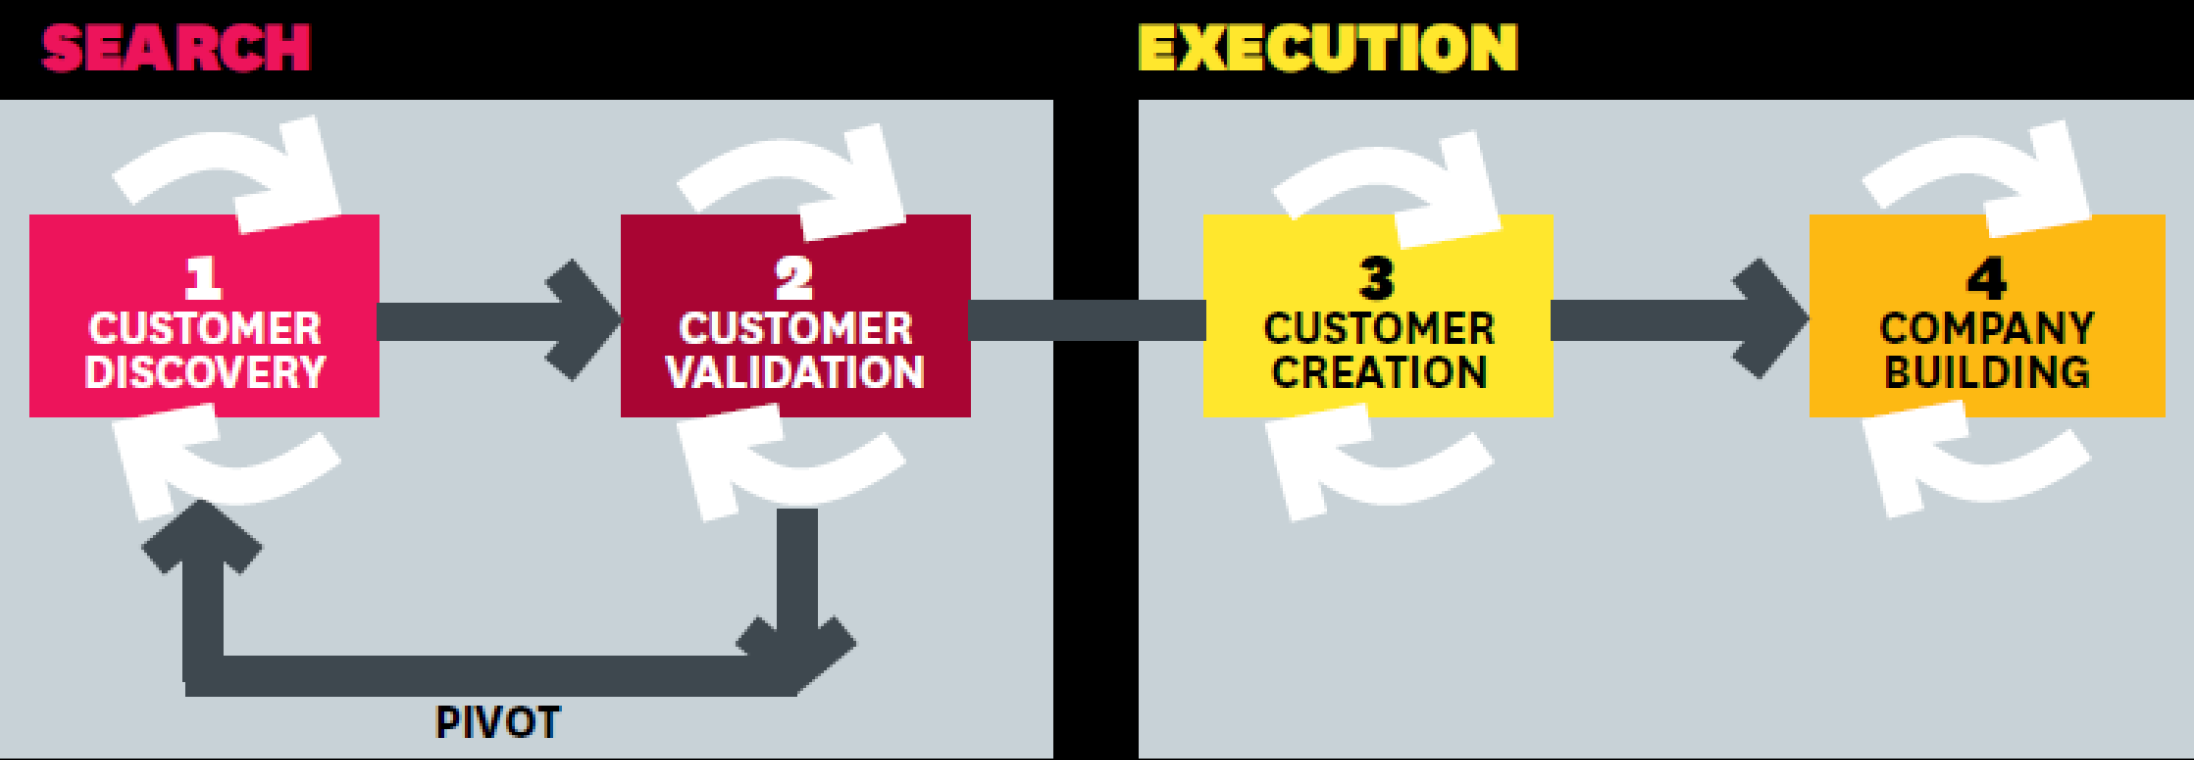
\includegraphics[width=1\linewidth]{images/lean_vorgehen}
	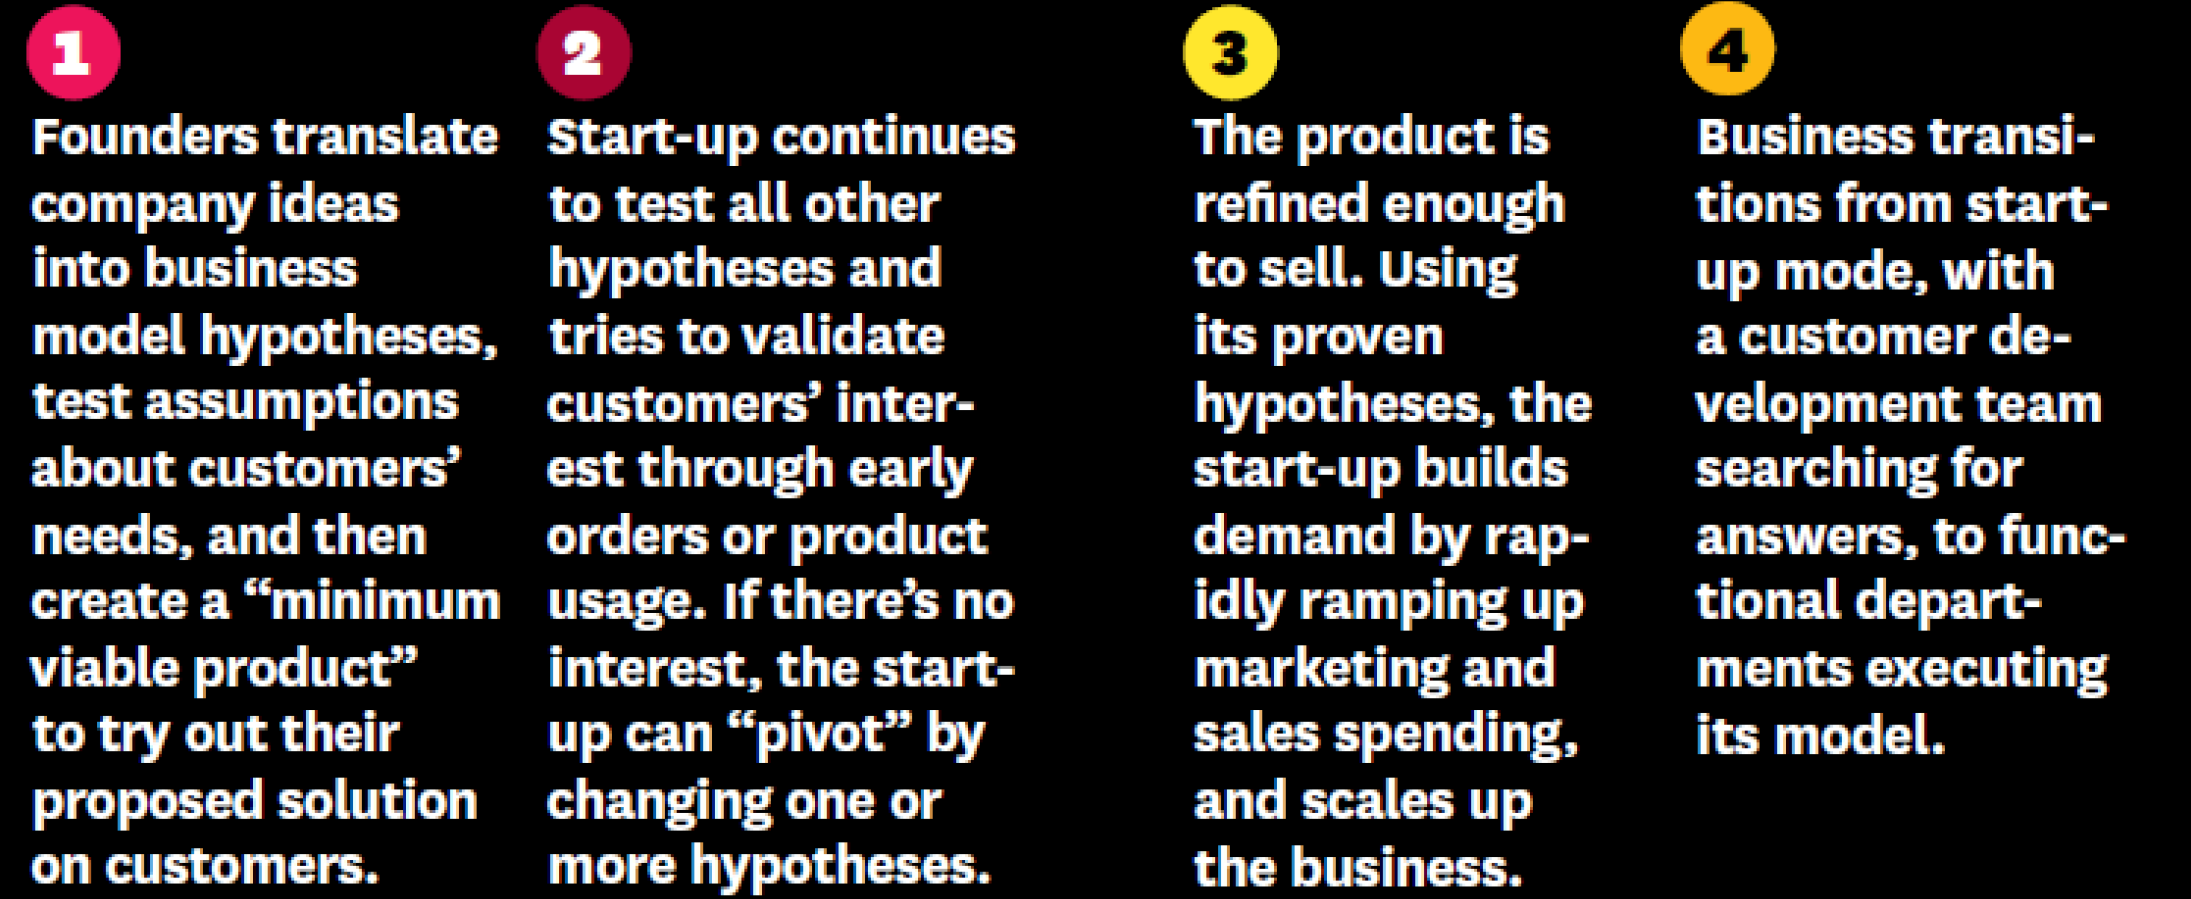
\includegraphics[width=1\linewidth]{images/lean_vorgehen_2}
\end{multicols}

\subsubsection{Minimum Viable Product (MVP)}
An MVP can be defined as the least amount of work we can do to in/validate a hypothesis, or problem a solution
is designed to solve.
\begin{itemize}
	\item Minimum: Small, earliest point to gather feedback
	\item Viable: Must have utility (e.g. not only the login feature)
	\item Product: Must be cohesive (e.g., not a random collection of features)
\end{itemize}
In contrast to traditional product development, in which each stage occurs in linear order and lasts for months, agile development builds products in short, repeated cycles. A start-up produces a “minimum viable product” - containing only critical features - gathers feedback on it from customers, and then starts over with a revised minimum viable product.

\subsubsection{What Successful Startups/Businesses Have in Common}
\begin{itemize}
	\item They started out doing A, testing A in the market, learning from the market reactions, and then pivoting to B
	\item Pivot = change directions but stay grounded in what we‘ve learned (Pivot = schnell anpassen)
	\item In order to succeed, you need to pivot quickly (i.e., before you run out of cash)
\end{itemize}
Beispiele:
\begin{itemize}
	\item Zoom-in Pivot In this case, what previously was considered a single feature in a product becomes the whole product. A zoom-in pivot, refocusing the product on what previously had been considered just one feature of a larger whole. (z.B. Instagram)
	\item Customer Need Pivot: The problem you’re trying to solve for them is not very important. However, because of this customer intimacy, we often discover other related problems that are important and can be solved by you. The target customer has a problem worth solving, just not the one that was originally anticipated. (z.B. PayPal)
	\item Business Architecture Pivot: a startup switches architectures. Some companies change from high margin, low volume by going mass market (e.g., Google’s search “appliance”); others, originally designed for the mass market, turned out to require long and expensive sales cycles.
\end{itemize}

\subsection{Pitching}
Whenever an entrepreneur presents information about his or her business, product or service he or she is pitching!

\subsubsection{Ziel}
The goal is to go one step further:
\begin{itemize}
	\item Generate attention
	\item Fix a next meeting
	\item Send a business plan or sales brochure
\end{itemize}

\subsubsection{Typen}
\begin{itemize}
	\item \textbf{„Elevator Pitch“ (30 seconds):} draw attention
	\item \textbf{Management presentations (5-10 minutes):} sell your project
	\item \textbf{Sales calls:} sell your product
\end{itemize}

\subsubsection{Regeln}
\begin{itemize}
	\item Keep it Simple (Brings auf den Punkt)
	\item Be Unique
	\item Be Enthusiastic
	\item Tell a Story (Roter Faden)
\end{itemize}

\subsubsection{Inhalt / Ablauf}
\begin{enumerate}
	\item Cover – One liner / Mission
	\item Problem
	\item Solution
	\item Market
	\item Business Model/ How to make money
	\item Competitors
	\item Go to Market
	\item Validation
	\item Team
	\item Demo	
\end{enumerate}